\documentclass[letter]{report}
% change draft to final when ready
% letter is US paper size 8.5 x 11.0 inches (215.9 x 279.4 mm)
% a4 is India/Europe 210 x 297 mm size

\newcommand\thesisTitle{MTech Thesis [Drafts] Template for AmritaU}
% title  of *your* thesis in Title Case

\usepackage[final]{graphicx}
% keep final to render figures; use draft to just have rectangles

\usepackage[usenames,dvipsnames]{color}
\PassOptionsToPackage{hyphens,obeyspaces,spaces}{url}
\usepackage{hyperref}
\hypersetup{
    pdftitle={\thesisTitle},
    pdfauthor={www.wright.edu/\~pmateti},
    pdfsubject={Latex and Theses},
    pdfkeywords=Latex and Theses,
    pdfcreator={emacs},
    pdfproducer={pdflatex},
    pdfnewwindow=true,
    colorlinks=true,        % false: boxed; true: colored
    linkcolor=blue,
    citecolor=Brown,
    filecolor=blue,
    urlcolor=Brown,
    bookmarks=true,
    unicode=false,
    pdftoolbar=false,
    pdfmenubar=false,
    pdffitwindow=true,
    pdfstartview={FitH},
}
\usepackage{algorithm2e}
\usepackage[square]{natbib}

% helpful macros while writing drafts of the proposal/ thesis
\newcommand\TBD[1]{\textcolor{red}{TBD~~#1}}
\newcommand\TBDMP[1]{{#1}\footnote{To be rewritten more precisely.}}
\newcommand\TBDMTBW{\quad More to be written.}
\newcommand\TBDFIG{{\vskip 2in}\footnote{Insert a figure here.}}
\newcommand\bumppages[1]{\addtocounter{page}{#1}}
\newcommand\KeepButNotInclude[1]{}

\newcommand\singleSpacing{\def\baselinestretch{1.0}}
\newcommand\doubleSpacing{\def\doubleSpacing{\def\baselinestretch{1.37}\normalsize}}


% LaTeX macros specific to this template example
\newcommand\TEX{\TeX{}}
\newcommand\tex{\TeX{~}}
\newcommand\web{{\tt WEB }}
\newcommand\latex{\LaTeX{~}}
\newcommand{\bibtex}{BiBTeX{~}}

\begin{document}

\pagestyle{plain}\newpage\pagenumbering{roman}\setcounter{page}{1}



\thispagestyle{empty}


\begin{center}

{\bf\Huge
Typesetting a Thesis/ Dissertation\\
Using Mateti's {\LaTeX} Example\\ %% title
}
\par\vskip 4cm

(\TBD{} For {\it this} document, the following is NOT true.)\\
A thesis submitted in partial fulfilment\\
of the requirements for the degree of\\
Master of Science in Computer Engineering\\  % replace

\par\vskip 2cm
By\\
\par\vskip 2cm


PRABHAKER MATETI\\              %% author name, all caps
B.S., Osmania University, 1970\\        %% previous degrees
M.Tech., Indian Institute of Technology at Kanpur, 1972\\
Ph.D., University of Illinois at Urbana-Champaign, 1976\\


\vfill

2016\\                          %% Year
Wright State University\\
Dayton, Ohio 45435-0001\\


\end{center}

\newpage


\newpage
\thispagestyle{empty}

\begin{center}
AMRITA SCHOOL OF ENGINEERING \\
AMRITA VISHWA VIDYAPEETHAM\\
\end{center}

\hfill
July 25, 2017\\			% DATE OF DEFENSE

I HEREBY RECOMMEND THAT THE THESIS PREPARED UNDER MY SUPERVISION BY
{\tt Sudip Hazra}		%% Full Name of the Student
ENTITLED
{\tt \thesisTitle}
BE ACCEPTED IN PARTIAL FULFILLMENT OF THE
REQUIREMENTS FOR THE DEGREE OF
{\tt Master of Technology in Cyber Security Systems and Networks}.\\


\hfill
\begin{minipage}{7cm}
\vskip 1cm\hrule\par\vskip 2mm
Prabhaker Mateti, Ph. D.\\	%%
Thesis Director\\
\vskip 1cm\hrule\par\vskip 2mm
Krishna Sri Achuthan, Ph.D.\\
Department Head\\
\end{minipage}

\vfill
\begin{minipage}{7cm}
Committee on\\
Final Examination\\
\vskip 1cm\hrule\par\vskip 2mm
Prabhaker Mateti, Ph. D\\
\vskip 1cm\hrule\par\vskip 2mm
Professor B, MTech or Ph. D\\
\vskip 1cm\hrule\par\vskip 2mm
Professor B, MTech or Ph. D\\
Professor C, MTech or Ph. D\\
\vskip 1cm\hrule\par\vskip 2mm
Krishna Sri Achuthan, Ph.D.\\
Dean, School of Graduate Studies
\end{minipage}

\newpage
\thispagestyle{plain}

{\centering\bf ABSTRACT\\}\par\vskip 2cm

\singleSpacing
\noindent
Subramanian, Sripriya.          %% last, first name, upper-lower case mix
M.S.  Department of Computer Science and Engineering,
Wright State University,
2003.                           %% this year
Sniffing the Ethernet with High Quality Tools. %% title

\par\vskip 2cm

\doubleSpacing

[This document is an example collection of files intended to help my
students in using LaTeX as they prepare their theses.  An abstract is
typically about one page.  The following is an example of an abstract
of a thesis.]

This thesis is a study of software quality in the limited context of a
class of network software tools called {\em sniffers}. Sniffers are
network monitoring tools used in the administration of network
security. We analyzed five of the hundreds of the existing sniffers to
determine the causes of poor quality and the methods to eliminate the
problems. We subjected the five selected sniffers to both manual
analysis and analysis by software quality assessment tools. We
classify the 1000+ errors so discovered in these sniffers. Based on
these results, we designed and implemented a new sniffer that is
intended as a model of high quality sniffer. The methods applied to
analyze and enhance the quality of software are studied.

Quality assessment software tools fall into two categories: 1) Static
checkers and 2) Dynamic checkers. Static checkers analyze the source
code. Dynamic checkers stand as guards during run-time. We have
collected and used exhaustively the checker tools that are in the open
source archives. In the course of our use, the quality of the software
quality tools is itself analyzed.

This thesis contributes several case studies of open source software
projects. It also contributes a new distributed sniffer to the open
source. The distributed sniffer can monitor multiple networks and
output desired packet details. We designed our sniffer to include a
MySQL based collector program, packet capture programs and viewer
programs. Our sniffer supports multiple capture and viewer
programs. We applied software engineering methods to eliminate the
quality issues associated with software. We use the results of our
analysis of existing sniffers in avoiding poor quality in our
sniffer. We prepared our sniffer for manual audit using documentation
tools. This new sniffer is an example of {\it literate programming}
that is worthy of study by software engineering students.

\newpage





\tableofcontents
\listoftables
\listoffigures
\newpage
\thispagestyle{plain}

{\centering\bf  ACKNOWLEDGEMENTS\\}\par\vskip 2cm

\singleSpacing
\noindent


\noindent
At the very outset, I would like to give the first honors to Amma, Mata Amritanandamayi
Devi who gave me the wisdom and knowledge to complete this minor project under her shelter
in this esteemed institution.
I express my gratitude to my guide, Prof. Prabhaker Mateti, Associate Professor, Com-
puter Science and Engineering, Wright State University, USA, for his valuable suggestion
and timely feedback during the course of this minor project.
I would like to thank Dr Krishnashree Achuthan, Professor and Head of the Center for
Cyber Security, for giving me useful suggestions and his constant encouragement and guidance
throughout the progress of this minor project.
I would like to thank my co-guides Mr. Vipin Pavithran, Assistant Professor, Cyber Secu-
rity, Amrita Vishwa Vidyapeetham for giving me useful suggestions and guidance throughout
the progress of this minor project.
I express my special thanks to my colleagues who were with me from the starting of the minor
project, for the interesting discussions and the ideas they shared. Thanks also go to my friends for sharing so many wonderful moments. They helped me not only enjoy my life, but also enjoy
some of the hardness of this minor project.

\vfill

\noindent


\doubleSpacing

\newpage





\pagestyle{headings}\newpage\pagenumbering{arabic}\setcounter{page}{1}

\chapter{Introduction}

Smartphones nowadays are capable of doing a multitude of tasks which was not possible with conventional phones, With the increase in complexity of smartphones, We can now send emails, click high-definition photos, Access satellite navigation and remain connected to the outside world 24 x 7.  The capabilities which makes smartphones different from conventional phones is giving nightmares to security organisations in tracing and extracting data from the smartphones.  The criminals are now  able to wipe out the traces of criminal activities performed using their phones with much ease than before.  The criminal organisations are also using smartphones to communicate with others using encrypted messages which are very hard to trace and decrypt.  Even if the phones are confiscated after the crime, It is becoming very hard for law-enforcement agencies to extract data from those devices as these devices are encrypted with advanced encryption features and any attempt to get access to the device memory using brute-force would potentially wipe the all the data inside and overwrite it with 0. In this scenario, A radically new approach is necessary to proactively monitor the criminal activities with minimal interference and maximum stealth.

\section{Smartphone OS Market Share}

According to Gartner ,it's estimated that there are roughly 2 billion smartphone users in the market (1.91 billion to be exact), with that number expected to increase another 12\% in 2016 to top 2.16 billion people globally. The global share of smartphone OS is as follows:

\begin{figure}
   \vspace*{-1cm}
    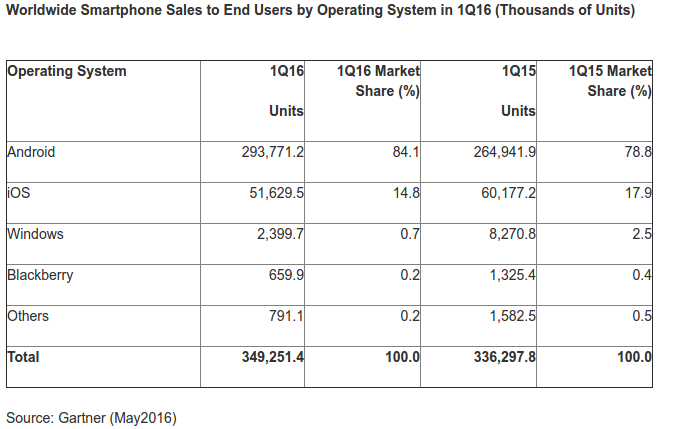
\includegraphics[height=0.5\textheight]{Figures/fig01/gartner}
    \caption{\href{http://www.gartner.com/newsroom/id/3323017} Gartner Survey Results}
    \label{gartner}
   
    
  \end{figure}


Android dominated the smartphone market with a share of 84 \% , IOS with 14.8 \% and Windows with 0.7\% of the Global smartphone market.As we can see Android OS is the most popular smartphone OS with almost 84 \% market share and hence we  are interested in examining the forensics capabilities in Android OS. 
\goodbreak
\section{Android Architecture}
Android is a mobile operating system developed by google based on the linux kernel and designed primarily for touchscreen mobile devices. Android source code is open-source and it is one of the main reason of the immense popularity of the android OS.
\begin{figure}
   \vspace*{-1cm}
    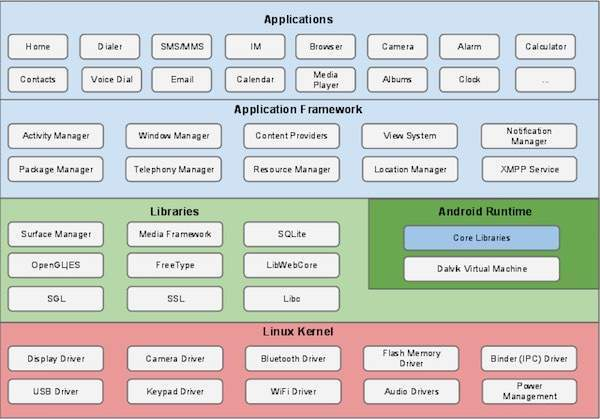
\includegraphics[height=0.5\textheight]{Figures/fig01/architecture}
    \caption{\href{https://www.tutorialspoint.com/android/}{Android Architecture} }
    
   
    
  \end{figure}


\subsection{Linux Kernel}
The basic layer is the Linux kernel. The whole Android OS is built on top of the Linux 3.x Kernel with some further architectural changes made by Google. It is this Linux that interacts with the hardware and contains all the essential hardware drivers. Drivers are programs that control and communicate with the hardware. For example, consider the Bluetooth function. All devices has a Bluetooth hardware in it. Therefore the kernel must include a Bluetooth driver to communicate with the Bluetooth hardware. The Linux kernel also acts as an abstraction layer between the hardware and other software layers. Android uses the Linux for all its core functionality such as Memory management, process management, networking, security settings etc. As the Android is built on a most popular and proven foundation, it made the porting of Android to variety of hardware, a relatively painless task.


\subsection{Libraries}
The next layer is the Android native libraries. It is this layer that enables the device to handle different types of data. These libraries are written in c or c++ language and are specific for a particular hardware.Some of the important native libraries include the following: 
\begin{itemize}

  \item \textbf{Surface Manager:} It is used for compositing window manager with off-screen buffering means you can't directly draw into the screen, but your drawings go to the off-screen buffer. There it is combined with other drawings and form the final screen the user will see. This off screen buffer is the reason behind the transparency of windows.

  \item \textbf{Media framework:} Media framework provides different media codecs allowing the recording and playback of different media formats.

  \item \textbf {SQLite:} SQLite is the database engine used in android for data storage purposes.

  \item \textbf{WebKit:} It is the browser engine used to display HTML content.

  \item\textbf{ OpenGL:} Used to render 2D or 3D graphics content to the screen.

  

\end{itemize}



\subsection{Android Runtime}

Android Runtime consists of Dalvik Virtual machine and Core Java libraries. 

\begin{itemize}

	\item \textbf{Dalvik Virtual Machine:}  It is a type of JVM used in android devices to run apps and is optimized for low processing power and low memory environments. Unlike the JVM, the Dalvik Virtual Machine does not run .class files, instead it runs .dex files. .dex files are built from .class file at the time of compilation and provides higher efficiency in low resource environments. The Dalvik VM allows multiple instance of Virtual machine to be created simultaneously providing security, isolation, memory management and threading support. It is developed by Dan Bornstein of Google. 

	Android 4.4 introduced Android Runtime (ART) as a new runtime environment, which uses ahead of time (AOT) compilation to entirely compile the application bytecode into machine code upon the installation of an application.

	

	\item \textbf{Core Java Libraries:} These are different from Java SE and Java ME libraries. However these libraries provides most of the functionalities defined in the Java SE libraries.

\end{itemize}

\subsection{Application Framework}

These are the blocks that our applications directly interacts with. These programs manage the basic functions of phone like resource management, voice call management etc.  Important blocks of Application framework are:

\begin{itemize}

\item \textbf{Activity Manager:}Manages the activity life cycle of applications.

\item \textbf{Content Providers:} Manage the data sharing between applications.

\item \textbf{Location Manager:} Location management, using GPS or cell tower .

\item \textbf{Resource Manager:} Manage the various types of resources we use in our Application.



\end{itemize}





\subsection{Applications}

Applications are the top layer in the Android architecture and this is where our applications are going to fit. Several standard applications comes pre-installed with every device, such as: 

\begin{itemize}

\item SMS client 

\item App Dialer

\item Web browser

\item Contact manager
\end{itemize}

\subsection{Applications Used in Criminal Activites}
The Criminals are increasingly becoming tech savvy and are using various apps which provide encryption facilities and as well as secure communication.This is becoming a problem for security agencies as they are not able to intercept the communication channel. .Some of the apps used by Criminals Networks are as follows:

\begin{itemize}
\item \textbf{Mappr} An App that can change location data on photos, so they don't reveal where they actually are.
\item \textbf{Cryptophone }An App that uses end-to-end encryption to for phone calls which effectively means that except the two communicating parties , no other person will be able the decrypt the data stream.
\item \textbf{Telegram} An  encrypted mobile messaging app that can host different channels where  members can talk in a group setting.
\item \textbf{Firechat} An App that connects to nearby devices which have firechat installed through wifi or bluetooth and build a "mesh network" that allows messages to be passed to other devices within vicinity without any usage of cell phone tower.
\end{itemize}


\clearpage

% -eof-

\chapter{Background}

Filesystems are collections of methods and data structures that an operating system uses to keep track of data on disks or partitions.Different operating systems uses different types of file systems like Windows uses NTFS and FAT32 file systems.Linux uses EXT4,EXT3,EXT2 etc.Earlier Android kernels used YAFFS2 file systems ,However newer Android kernels use EXT4 file systems.File systems atre implemented at kernel level.Implementing a new file system at the kernel level involves modifying the kernel source code and rebuilding it with the new file system support,This creates complexity which can be solved by implementing file system at the user level .
\section{Fuse(File system in User Space)}
\begin{figure}[H]
   
    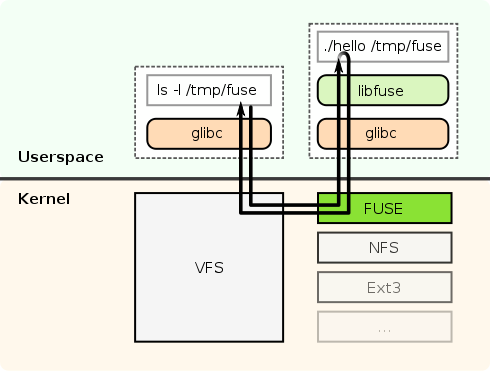
\includegraphics[width=0.7\textwidth ]{Figures/fig02/fuse}
    \caption{\href{https://en.wikipedia.org/wiki/Filesystem_in_Userspace}{Filesystem in Userspace }} 
  \end{figure}
FUSE (Filesystem in Userspace) is an interface for userspace programs to export a filesystem to the Linux kernel. The FUSE project consists of two components: the fuse kernel module  and the libfuse userspace library . FUSE is particularly useful for writing virtual file systems. Unlike traditional file systems that essentially save data to, and retrieve data from, mass storage, virtual filesystems do not actually store data themselves. They act as a view or translation of an existing file system or storage device. FUSE has a small kernel module  which plugs into the VFS layer in the kernel as a file system and then communicates with a user-level process that does all the work, using the FUSE library to communicate with the kernel module. IO requests from an application are redirected by the FUSE kernel module to this user level process for execution and the results are returned back to the requesting application.
\linebreak
A fuse file system is a user-space program that listens on a socket for file operations to perform and perform them. The fuse library(libfuse) provides the communication with the socket and passes the requests to the code.The callbacks are a set of functions to implement the file operations and a struct fuse\_operations contains pointers to them.\\




Necessary operations in fuse\_operation structure \cite{Writing_a_FUSE_Filesystem}\\
struct fuse\_operations \{
\begin{itemize}

\item  int (*getattr) (const char *, struct stat *);

\item int (*readlink) (const char *, char *, size\_t);

\item int (*getdir) (const char *, fuse\_dirh\_t, fuse\_dirfil\_t);

\item int (*mknod) (const char *, mode\_t, dev\_t);

\item int (*mkdir) (const char *, mode\_t);

\item int (*unlink) (const char *);

\item int (*rmdir) (const char *);

\item int (*symlink) (const char *, const char *);

\item int (*rename) (const char *, const char *);

\item int (*link) (const char *, const char *);

\item int (*chmod) (const char *, mode\_t);

\item int (*chown) (const char *, uid\_t, gid\_t);

\item int (*truncate) (const char *, off\_t);

\item int (*utime) (const char *, struct utimbuf *);

\item int (*open) (const char *, struct fuse\_file\_info *);

\item int (*read) (const char *, char *, size\_t, off\_t, struct fuse\_file\_info *);

\item int (*write) (const char *, const char *, size\_t, off\_t,struct fuse\_file\_info *);

\item int (*statfs) (const char *, struct statfs *);

\item int (*flush) (const char *, struct fuse\_file\_info *);

\item int (*release) (const char *, struct fuse\_file\_info *);

\item int (*fsync) (const char *, int, struct fuse\_file\_info *);

\item int (*setxattr) (const char *, const char *, const char *, size\_t, int);

\item int (*getxattr) (const char *, const char *, char *, size\_t);

\item int (*listxattr) (const char *, char *, size\_t);

\item int (*removexattr) (const char *, const char *);

\};

\end{itemize}

\begin{figure}[H]
   \centering
    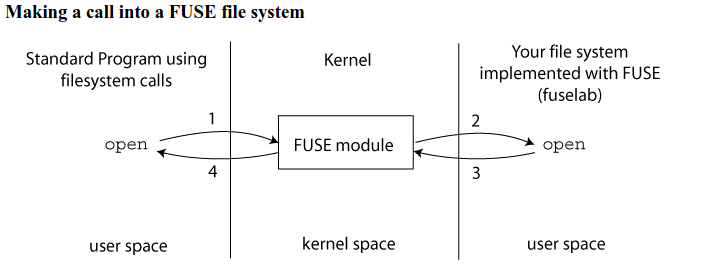
\includegraphics[width=0.7\textwidth ]{Figures/fig02/workingfuse}
    \caption{\href{https://www.cs.cmu.edu/~fp/courses/15213-s07/lectures/15-filesys/}{Making a Call in Fuse File System} } 
  \end{figure}


\textbf{Example of Fuse Filesystems:\cite{wiki:Filesystem_in_Userspace}} 
\begin{itemize}

\item \textbf{CloudStore (formerly, Kosmos filesystem):} By mounting via FUSE, existing Linux utilities can interface with CloudStore
\item \textbf{EncFS:} Encrypted virtual filesystem
\item \textbf{ExpanDrive:} A commercial filesystem implementing SFTP/FTP/S3/Swift using FUSE
\item \textbf{GDFS:} Filesystem which allows you to mount your Google Drive account on Linux.

\item \textbf{GlusterFS:} Clustered Distributed Filesystem having ability to scale up to several petabytes.
\item \textbf{GmailFS:} Filesystem which stores data as mail in Gmail.
\item \textbf{GVfs:} The virtual filesystem for the GNOME desktop.
\item \textbf{KBFS:} A distributed filesystem with end-to-end encryption and a global namespace that uses FUSE to create cryptographically secure file mounts.
\item \textbf{MooseFS:} An open source distributed fault-tolerant file system available on every OS with FUSE implementation (Linux, FreeBSD, NetBSD, OpenSolaris, OS X), able to store petabytes of data spread over several servers visible as one resource.
\item \textbf{NTFS-3G and Captive NTFS:} allowing access to NTFS filesystems.
\item \textbf{Sector File System:} Sector is a distributed file system designed for large amount of commodity computers. Sector uses FUSE to provide a mountable local file system interface.
\item \textbf{SSHFS:} Provides access to a remote filesystem through SSH.
\item \textbf{Transmit:} A commercial FTP client that also adds the ability to mount WebDAV, SFTP, FTP and Amazon S3 servers as disks in Finder, via MacFUSE.
\item \textbf{WebDrive:} A commercial filesystem implementing WebDAV, SFTP, FTP, FTPS and Amazon S3.
\item \textbf{WikipediaFS:} View and edit Wikipedia articles as if they were real files.
\item \textbf{Wuala:} A multi-platform, Java-based fully OS integrated distributed file system. Using FUSE, MacFUSE and Callback File System respectively for file system integration, in addition to a Java-based app accessible from any Java-enabled web browser.
\end{itemize}

\section{Cloudfs}
CloudFS will be developed using the file system in user-space (FUSE) toolkit. FUSE provides a framework for implementing a file system at user level.  CloudFS will be implemented  as user-level code that uses libfuse to communicate with  applications  and uses regular file system calls  to access the storage. By default, FUSE is multi-threaded, so multiple system calls from user applications can be running at the same time in the user-level process, allowing higher parallelism and  faster performance. Cloudfs can be used to mount cloud storage like dropbox, google drive and onedrive as local file system and any changes that are made in the local file system are syncronised with cloud storage. For example :
\begin{itemize}
\item WingFS, the universal cloud adapter, mounts the cloud service on the desktop.Storage services can be used  like a hard drive without the need for apps, specific folders, browser plug-ins and login processes.
\item Google Cloud Storage Fuse: It is an open source fuse adapter that allow us to mount Google cloud storage buckets as file systems on Linux or OS X systems. It also provides a way for applications to upload and download google cloud storage objects using standard file system semantics. It is written in Go language and hosted in github.
\item The Storage Made Easy Linux App Suite is comprised of an integrated Cloud Drive (that uses FUSE), a graphical Cloud File Explorer and also Sync tools to sync cloud files to/from the Linux desktop.
\item Drop-Fuse is a simple fuse based file system which is written in python and can mount the dropbox drive as local file system in Linux.


\end{itemize}
In our case We will be implementing the cloud fs below the android software stack in linux level and api's will be used synchronization and mounting a multitude of cloud storage services.
\section{Stealthfs via Rootkits}
When we  install a rootkit in that system we will be able to get administrator privileges whenever you want. Good rootkits can hide in compromised system, so that they can't be found by administrator. There are many ways to hide in a system.For example there are rootkits that replace some most important programs in system(ls, ps, netstat etc.) with modified versions of them that won't let administrator see that something's wrong. Although, such a rootkit is quite easy to detect. Other rootkits work as linux kernel modules. They work in kernel mode, so they can do everything they want. They can hide themselves, files, processes etc.\\
\linebreak
\bigskip 
Different types of Rootkits are explained below.
\subsection{User Level Rootkits}

User level rootkits are unprivileged and are stored outside of kernel memory
 space. They are user space code that patches or replaces existing applications to provide
 cover for malicious activities. User level rootkits replace system binaries, add malicious
 utilities, change configuration files, delete files, or launch malicious processes.For example, the Linux system program ‘ls’ could be changed so as to not reveal the
 presence of a malicious file in a directory. These rootkits, while effective, are easily
 detected by file system integrity and signature checking tools , therefore, most
 modern IDS software prevent these rootkits from being installed or can detect an active
 intruder.

\subsection{Kernel Level Rootkits}
Kernel level rootkits defeat such tools by directly modifying the operating system
 kernel. These rootkits modify the execution flow of kernel code to run their own payload.
 However, modifying the kernel in this way can drastically affect the stability of the
 system causing a kernel panic.

The simplest way to introduce code into a running kernel is through a Loadable
 Kernel Module (LKM) . LKMs add flexibility to an operating system by
 providing a means to add functionality without recompiling the entire kernel. Added
 functionality might include device drivers, filesystem drivers, system calls, network
 drivers, TTY line disciplines, and executable interpreters . Most modern UNIX-
like systems, including Solaris, Linux, and FreeBSD, use or support LKMs.
However, the kernel packaged with Android does not support LKMs by default. The
 kernel can be recompiled and installed on Android to add LKM support if physical access
 to the mobile is available. LKMs are very useful, but they also allow maliciously written
 kernel modules to subvert the entire operating system which can lead to a loss of control
 of the Linux kernel and consequently all the layers above the kernel . Kernel level
 rootkits typically subvert the kernel to hide processes, modules, connections and more to
 avoid detection. Particular techniques include hooking system calls, direct kernel object
 manipulation (DKOM), run-time kernel memory patching, interrupt descriptor table
 hooking, and intercepting calls handled by Virtual File System (VFS). These techniques
 are discussed at a high level in this section.


\subsubsection{Hooking System Calls}
The kernel provides a set  of  interfaces or system calls by which processes running
 in user space can interact with the system. The applications in user space send requests
 through this interface and the kernel fulfills requests or returns an error. Hooking is a technique that employs handler function, called hooks, to modify
 control flow . A new hook registers its address as the location for a specific
function, so when that function is called the hook runs instead. Typically, a hook will call
 the original function at some point to preserve the original behavior. System calls can be
 hooked using a maliciously designed LKM to alter the structure of the system call table.

\subsubsection{Direct Kernel Object Manipulation (DKOM)}
Hooking the system write call allows a rootkit to hide from system binaries like
 ls, lsmod, and ps; even so, robust IDSs can still detect the existence by following the
 kernel structures. All operating systems store internal record-keeping
 keeping data in main
 memory . The Linux kernel is no exception and provides generic data structures
 and primitives to encourage code reuse by developers . These structures, that all
 programmers are familiar with, include linked lists, queues, maps, and binary trees.
 Altering the data in these structures to hide an attacker’s activity is called Direct Kernel
 Object Manipulation (DKOM).

\subsubsection{Interrupt Descriptor Table (IDT) Hooking}
An interrupt is an event that alters the sequence of instructions executed by the
 processor. When an interrupt occurs a system table called the Interrupt Descriptor Table
 (IDT) associates each interrupt or exception with the address of the corresponding
 handler . System calls use software interrupts to switch from user mode to kernel
 mode. The interrupt handler invokes the system call handler from the address stored in
 the system call table. A rootkit can hook the IDT by modifying the interrupt handler
 address in the IDT or by patching the first few instructions of the interrupt handler
.These modifications would put the rootkit code in the flow of execution while
 still letting the system handle interrupts properly.
\chapter{Problem Statement}
\label{chap:problem statement}

The project is a part of an ongoing project on Proactive Forensics. The Previous Work has been done by Karthik Et.al \cite{Karthik2016} and  Aiyyappan Et.al \cite{Aiyyappan2015}. Aiyyappan ported the inotifywait to android. File events are tracked by inotify tool and the inotify source was complied using NDK programming and compiled to a native shared object library. The native function excepts a directory to track and all file events are tracked. He also created the forensic examiner toolkit which runs on linux machine to image, recover and collect device specific data from the cloud. Some amount of stealth was also enabled using hidepid =2 , where users can only see their own processes and process id's are also hidden from /proc also.

Karthik created the android apk which extensively tracks the user activities like GPS,Sensor data,WIFI Metadata,Sms,Call recording and keylogger was also included in the apk , which could be configured when the rom is flashed and used for the first time, after that there is no dialog whatsoever and the app runs in stealth mode and saves all the forensically relevant data in/forensic partition and opportunistically uploads it to the cloud.However the background process can be discovered if the user roots the phone and gets root access , Then he /she can easily see all the background process running and can also discover the /forensic partition , compromising the evidence , even though the partition is encrypted but it will still create suspicion in the suspects mind. 
\newpage
\section{Aim}
There are two possible solutions in this scenario:\\
\begin{itemize}
\item 1. The /forensic partition can either be encrypted and stored in the device,However it may led to suspicion as the user will be able to read all data except that partition.\\

\item 2. Another solution is to create A Fuse File System and store the forensically relevant data in that file system.The file system can then be hidden using rootkits which will subvert commands such as df and du and prevent any normal user for detecting the file system.

\end{itemize}
\bigskip

The Proposed Framework Will be Consisting of:\\
\begin{itemize}
\item An EXT4 file system which will store the forensically relevant data from the device.The forensic service designed by  Karthik \cite{Karthik2016} and Aiyappan \cite{Aiyyappan2015} will store all the user data obtained from the device in this file system.

\item An user space file system based on FUSE library which will mount the cloud storage as a local drive in the device accessible to the forensic service.The cloud drive will support major cloud storage service providers and will be configurable using an apk and an config file. The stealth file system will copy itself piece by piece to the cloud file system which will then opportunistically upload it to the cloud storage.This will give more storage for the forensic service to store greater amount of evidence in comparison to limited amount of device storage.

\item A kernel level android rootkit which will hide both the EXT4 File system and the cloud file system from typical linux command like df,du and mount commands by hooking the sys\_call\_table and subverting the systems calls.

\item Combining All the above we get a stealth file system with cloud file system support which will be mounted below the android software stack in the linux level.
 
\end{itemize}
\bigskip

Advantages of Mounting The cloud storage as local file system:
\begin{itemize}
\item We will be able to do all file system operations possible such as create, delete, modify files and directories.
\item All applications will see the mounted cloud storage as local storage and will be able to perform all operations possible with a local file system.
\item The storage capacity will increase manifold, typical modern android devices have storage capacity of maximum 64GB however if we are mounting the cloud drive as local storage , we are potentially having unlimited access to the storage . The storage capacity will increase manifold with terrabytes of storage space.
\item The Android Cloud Storage Service(ACCS) will also be employed in our companion projects :\\
\tt 
1.Detecting Trojans in Android Devices by Manuel Antony.\\
\tt 

\end{itemize}


\chapter{Stealth File System with Cloud Support}
\label{chap:proposal}

Here we propose a Stealth File system with cloud support  Below the Android  Software stack.
\begin{figure}[h]
   \centering
   \includegraphics[width=15cm]{Figures/fig04/FUSE}
   \caption{Proposed System Architecture}
  \end{figure}
 \section{ Modules Description:}
 
\subsection{Forensic Service}
The forensic service designed by Karthik\cite{Karthik2016} Et.al and Aiyyappan Et.al\cite{Aiyyappan2015} will collect the forensically relevant data from the device partitions and will send it to the /forensic file system. The data sent will include:
\begin{itemize}
\item Phonebook\\
  com.android.providers.contacts/databases/contacts2.db
\item Call History\\ com.android.providers.contacts/databases/contacts2.db
\item Browsing History\\ com.android.browser/databases/browser.db
\item Calender\\ com.android.providers.calendar/databases/calendar.db
\item SMS com.android.providers.telephony/databases/mmssms.db
\item WhatsApp\\ com.whatsapp/databases/msgstore.db
\item GMail\\ com.google.android.gm/mailstore.<username>@gmail.com.db

\textbf{In addition to these Data Keylogger data ,call record data and Sensor data will also be sent to the forensic partition.}
\end{itemize}
  \subsection{Stealth File Systems}
  The stealth file system will be a seperate file system which will be used by the forensic service to copy all the forensically relevant data from the relevant device partitions like /data to the stealth file system. The stealth file system will be based on ext4 file systems, rootkits will be used to hide the file volumes from commands like df and du. The rootkit will be responsible for subverting systems calls which can potentially expose the presence of the either the forensic service running or the stealth file system and the cloud file system.The rootkit will also hide the forensic service running in the background by hooking on to the sys\_call\_table and filtering out the output. In future the stealth file system will be based on a seperate emmc partition for added stealth.
  \subsection{Cloud File System}
  The cloud File system will made using fuse , and we will be able to locally mount a cloud drive as the cloud file system. It will support various cloud providers using api's .The cloud drive will opportunistically upload the data to the cloud storage online. The cloud file system will also be made stealth using rootkits and seamlessly copy data from the stealth file systems and sync it .It will also act a cache to prevent data loss.\\
  
  Cloud Drives can be mounted as Local Drives using the various cloud storage provider api's like:\\
  \textbf{Cloud Storage API's Examples:}\\
  Dropbox Cloud Storage Api's:\\
  \begin{itemize}
  \item Create a Dropbox folder \\
  \tt post('https://api.dropbox.com/1/fileops/create\_folder', args)\\
  \item Rename a Dropbox file/directory object.\\
    \tt  post('https://api.dropbox.com/1/fileops/move', args)\\
    
   \item Delete a Dropbox file/directory object.\\
    \tt post('https://api.dropbox.com/1/fileops/delete', args)\\
    
    \item Get Dropbox metadata of path.\\
    \tt
    get('https://api.dropbox.com/1/metadata/auto' + path, args)\\
  
  \end{itemize} 
 	
  
  
 
  
  As per the official android documentation the external storage (SD cards) are accessed by the Android system using FUSE which implies that FUSE is supported by the kernel directly so we dont need to add fuse support in kernel , we need to develop the cloudfs which will be controlled by the Android Cloud Storage Service(ACCS)  which will run as a background service and will be configurable using an Apk and .config file.The stealth file system with the cloud file system will work with forensic service developed by aiyyappan and karthik and will be incorporated into the forensic rom.
  
  

\chapter{Results and Discussion}
\label{chap:results}
The Following implementation have been done on Ubuntu Linux and our objective is to implement the framework in a Linux environment and then port it to Android.

\section{Fuse File System in Linux}

To develop a filesystem, first download the FUSE source code https://github.com/libfuse/libfuse/releases  and unpack the package This creates a FUSE directory with the source code. The
contents of the fuse directory are:
\begin{itemize}
\item ./doc contains FUSE-related documentation. At this point, there is only one file, how-fuse-
works.
\item  ./kernel contains the FUSE kernel module source code .
\item  ./include contains the FUSE API headers, which  needed to create a filesystem. The only
one you need now is fuse.h.
 \item ./lib holds the source code to create the FUSE libraries to link binaries to create a filesystem.
\item ./util has the source code for the FUSE utility library.
 \item ./example, of course, contains samples for your reference, like the fusexmp.null and hello
filesystems.\\
\end{itemize}
\textbf{Build and install FUSE:}\\
1. Run the configure script from the fuse-2.2 directory: ./configure . This creates the required
makefiles, etc.\\
2. Run ./make to build the libraries, binaries, and kernel module. Check the kernel directory for
the file ./kernel/fuse.ko -- this is the kernel module file. Also check the lib directory for fuse.o,
mount.o, and helper.o.\\
3. Run ./make install to complete the installation of FUSE.\\

\textbf{Fusepy}\\
fusepy is a Python module that provides a simple interface to FUSE\_ and
MacFUSE\_. It's just one file and is implemented using ctypes.
\section{Mounting a Demo Fuse File System in Python}
\begin{figure}[h]
   \centering
   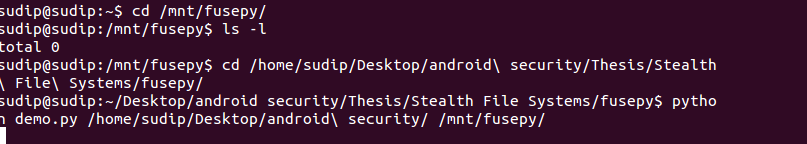
\includegraphics[width=15cm]{Figures/fig05/fusepy}
   \caption{Mounting a Fuse File System}
   
  \end{figure}
  \begin{figure}[h]
     \centering
     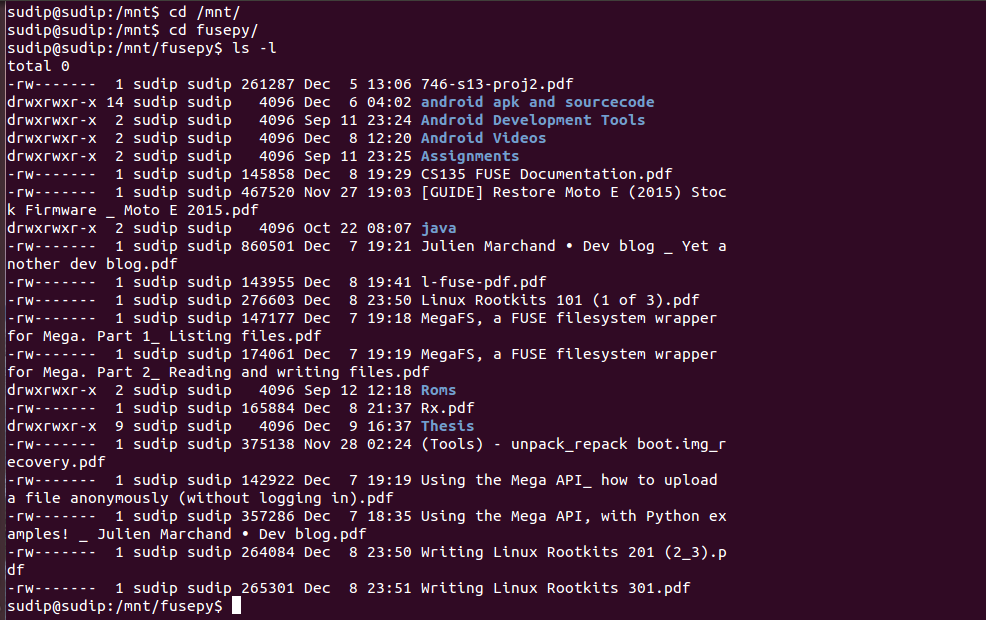
\includegraphics[width=15cm]{Figures/fig05/mnt}
     \caption{Contents of the Mounted File System}
     
    \end{figure}
    
    
\vspace{2cm}    
\section{Mounting a Cloud Drive as Local File System}



\subsection{\href{https://github.com/matteoserva/MegaFuse}{MegaFuse}}
This is a linux client for the MEGA cloud storage provider. It is based on FUSE and it allows to mount the remote cloud drive on the local filesystem. Once mounted, all linux program will see the cloud drive as a normal folder.\\

This software is based on FUSE.\\

\begin{figure}[h]
   \centering
   \textbf{Megafs.h  header Information}
   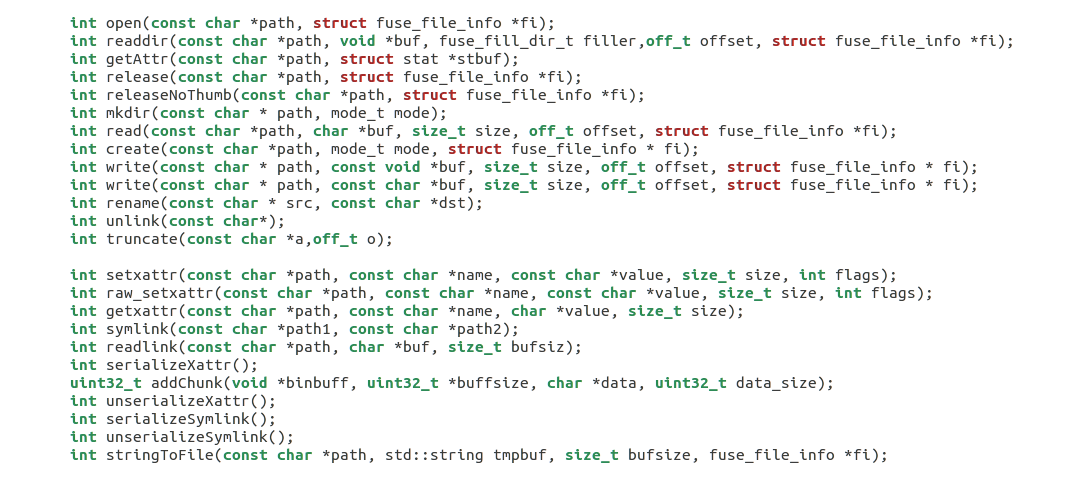
\includegraphics[width=12cm]{Figures/fig05/mega1}
   \caption{Megafuse.h defining supported  Fuse File Operations}
    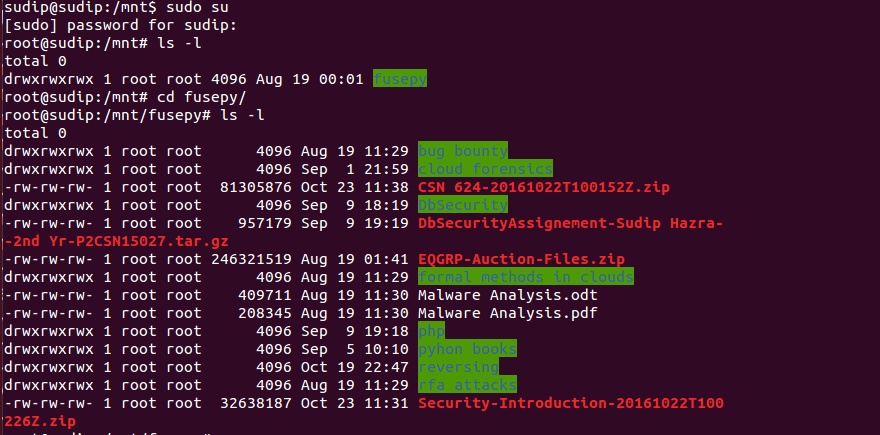
\includegraphics[width=12cm]{Figures/fig05/mega2}
                  \caption{Mounted Megafuse Cloud Drive}
   
  \end{figure}

\begin{figure}[h]
   
   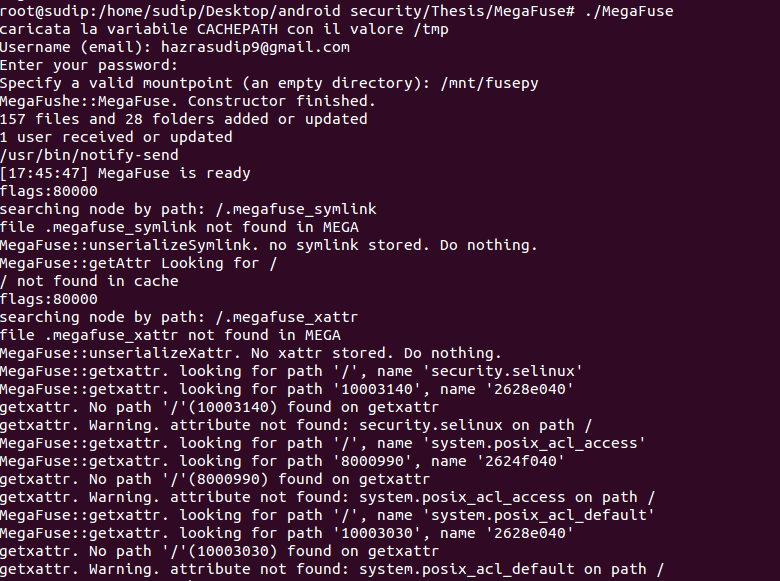
\includegraphics[width=15cm]{Figures/fig05/mega4}
   \caption{Running Megafuse Client}
   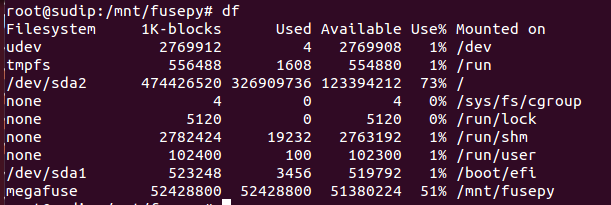
\includegraphics[width=15cm]{Figures/fig05/mega3}
        \caption{ Megafuse File System as seen by df command}
       
   
  \end{figure}

  
\section{Evidence Recovery using Sleuthkit Forensic Recovery Tool}
Sleuthkit \cite{Sleuthkit} is an open-source Forensic Recovery toolkit capable of recovering forensic artifacts from device memory image.We used an android device for 1 week and then made factory reset , and created an image of device using dd command and ran sleuthkit over it to recover artifacts.\\

\subsection{Results}
\begin{figure}[h]
   \centering
   \textbf{Running Sleuthkit Forensic Toolkit}\\
   \bigskip
   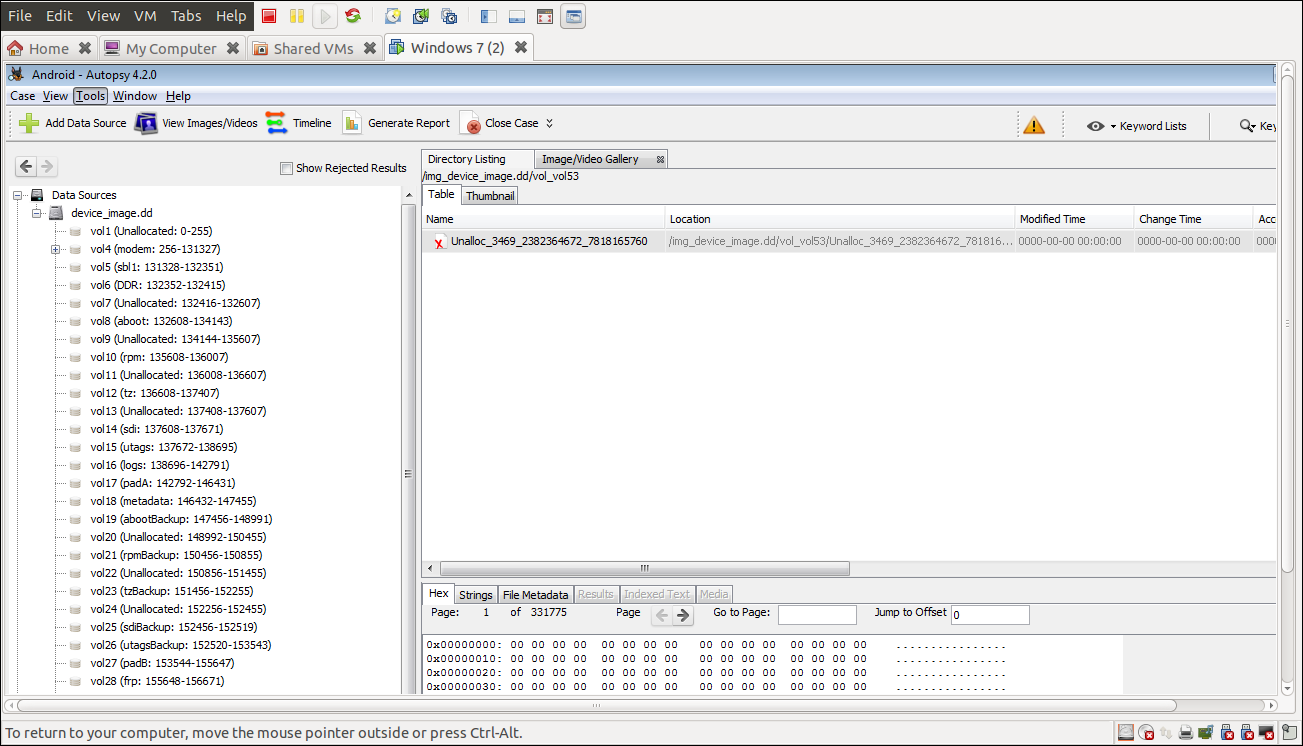
\includegraphics[width=12cm]{Figures/fig05/sleuthkit}
   \label{Sleuthkit Forensic Toolkit}
   \caption{Device image Analysis using Sleuthkit}
 \end{figure}
\begin{figure}[h]
\centering
\textbf{Recovered Images}\\
 \bigskip
  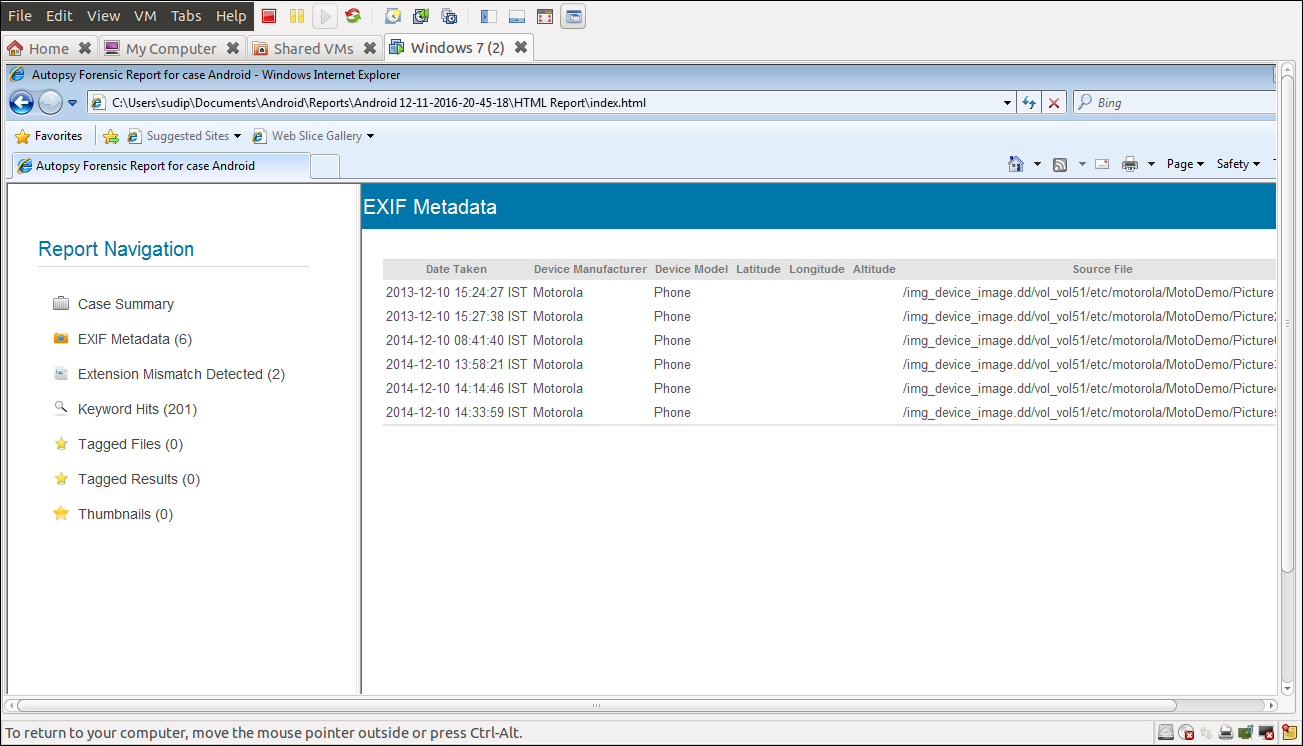
\includegraphics[width=12cm]{Figures/fig05/exitmetadata}
  
\caption[Recovered Images]{Very Few Images Could be Recovered After Factory Reset of device}
\end{figure}

\begin{figure}[h]

\centering
\textbf{Recovered Email Id's}\\
    \bigskip
    
       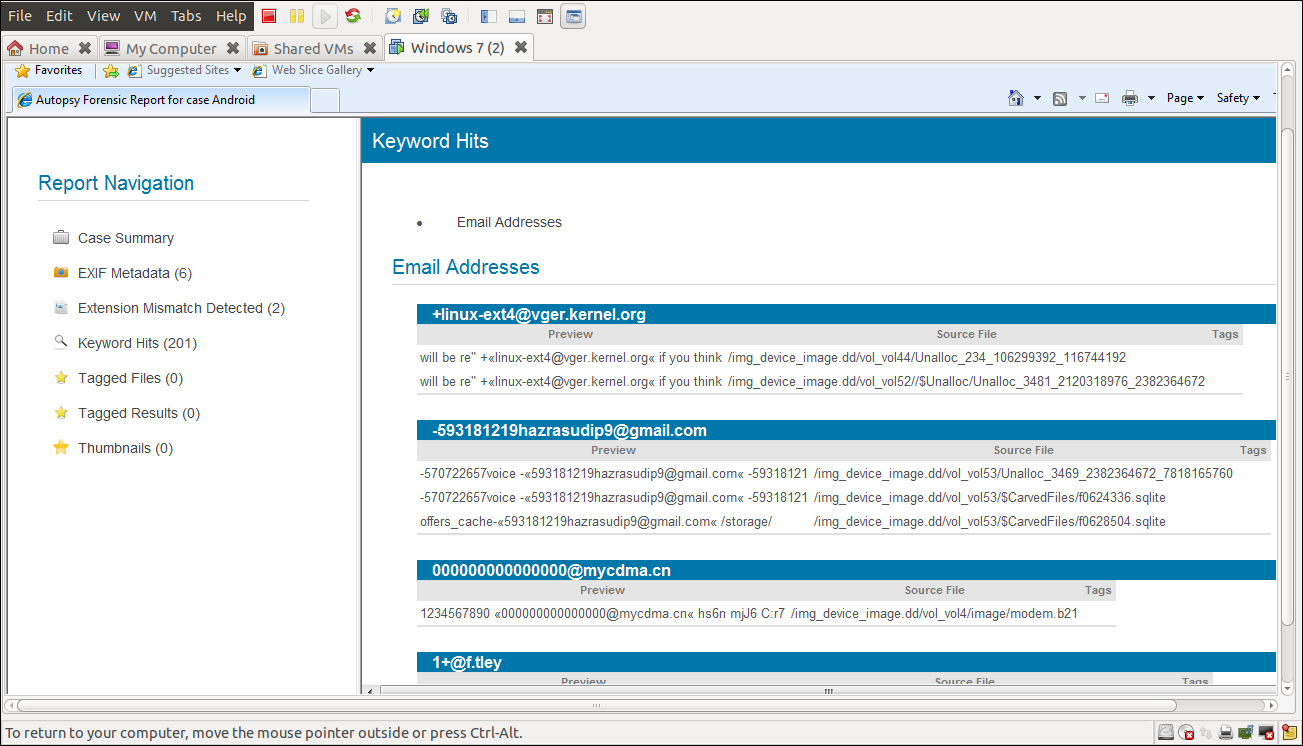
\includegraphics[width=12cm]{Figures/fig05/emails}
       \label{Email Recovery with Sleuthkit}
       \caption[Recovered Emails]{Very Few Emails Could be recovered after Factory Reset of device}
\end{figure}
\bigskip


\section{Hiding File Systems Using Rootkits}
A Rootkit can be hidden by finding out the location of the sys\_call\_table and hijack  write  with  our  own  write function. We'll first want to save a copy of the original write to pass data off to and restore when the module is unloaded.To do this we'll simply use the xchg() function and exchange the two pointers. 


\begin{figure}[h]

\centering
\textbf{Hiding Filesystems using Rootkits}\\
    \bigskip
    
       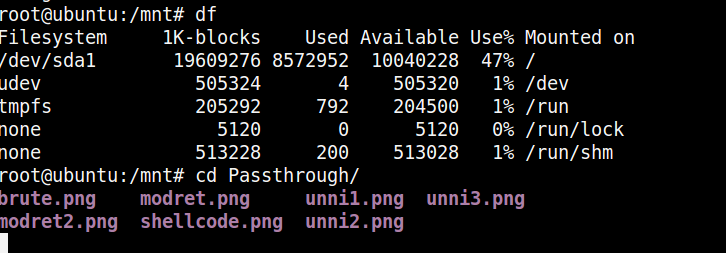
\includegraphics[width=12cm]{Figures/fig05/rooty}
       \caption[Hiding Filesystem Using Rootkits]{The write system call is highjacked, However the filesystem is still mounted.}
\end{figure}




    
 









  




\chapter{Related Work}
\label{chap:lit_review}
The Following is Collection of Literature Review on Works related to Android Forensics and other articles related to our area of interest.\\
\bigskip 

\textbf{Androphsy: Forensic Framework for Android }\\
\cite{akarawita_2015}  implemented a forensic framework which can acquire data both 
Physically and logically from the android smartphone. For physical acquisition they 
used DD program to clone the system image. For logical acquisition they use adbpull 
to clone the filesystem partition, other tools used were logcat,demsg ,dumpsys,scalpel 
and adb getprop to get device properties.Used Netcat to copy the system files to a 
remote server. It was better than other Opensource Forensic tools like Oxygen and 
ViaExtract CE tool. Rooting of the phone is necessary.\\

\textbf{Smartphone Forensics : A proactive Investigative Approach}\\
\cite{mylonas2012} suggested a proactive forensic framework which is regulated by an 
independent authority. Two modes of forensics namely Usermode and Network 
mode. No information about Implementation , was the phone rooted or unrooted, 
functionality of the app not given.\\ 

\textbf{Frost: Forensic Recovery of Scambled Telephones}\\
\cite{muller2013frost}deviced an forensic image which was flashed on to the phone and it was 
capable to bruteforcing Pin, direct recovery of encryption keys and decrypting user 
partition on phone itself. If the bootloader is locked not of much use , only option is 
to take memory dump but all smartphones now comes with default locked bootloader, secondly only if the handset is instantly available to the expert , he can freeze the ram to minimize 
data loss and recover encryption keys from ram.\\

\textbf{Android Forensics : Automated Data Collection and Reporting Tool for Mobile Device }\\
Justin Grover \cite{Grovera2013} made the first of its kind android forensics tool which collected data with user consent and uploaded it to a remote server. The capabilities are limited and are susceptible to tampering . Droidwatch mainly uses content observers,Broadcast Receivers and Alarms for monitoring. Broadcast Receivers and Alarms can be tampered with. No data about social networking apps , no support was there for email. \\


\textbf{Specifying a Realistic File System }\\
 Bilbyfs \cite{amani2015specifying}   is a an asynchronous write flash file system whose formal verification is done using Isabelle/Hol. The file system needs a C-Wrapper which is placed between the VFS and the filesystem hence direct mapping is not possible. which can be a disadvantage. It follows strict ordering of updates and do not support concurrency. It was formally verified that the Bilbyfs indeed follows async writes .\\

\textbf{A Fast Boot, Fast Shutdown Technique for Android OS Devices}\\
The paper \cite{yang2016} demonstrates a new technique of Fast Boot in android called FBFS. Here the snapshot is taken of the system only once and hence afterwards whenever the system boots, it makes a call to RSS\verb+\+\_thread to sync the ram image with the latest files in emmc. significantly decreases the startup time to 7.8secs and shutdown to normal 10.3 secs, but when will the system know when to update the snapshot upon system update or a specified amount of time is not addressed.\\

\textbf{Internet-Scale File Analysis}\\
A \cite{hanif2015} large scale malware analysis framework implemented in skald framework and has loosely coupled components like transporter ,planner and services, all inter-connected but highly failure resistant. TOTEM is the name of the tool tey created using the framework, written in scala using AKKA. Planner designates tasks to various services which execute and the reports are forwarded using RabbitMQ messaging protocol . Highly concurrent and a very good technique for mass scale malware analysis but more details are needed how the service outputs are fed to humans or scripts for report generation.\\


\textbf{Subverting Operating System Properties Through Evolutionary DKOM Attacks}\\
 New type \cite{graziano2016} of DKOM attack ,does not change the kernel dynamic data structures at once but continues to do it over a period of time. Difficult to detect because there is no sudden change but continuous one. attacks the cfs tree of the scheduler but not the process tree hence the app being attacked shows in the ps but it is indefinitely delayed in the scheduler as the vruntime is set to max. Detected using a thin hypervisor debugger which uses defensive mimic technique to detect the attack using periodic monitor and task tracker. Can stop ids or any antivirus and do not modify kernel code. Various other variation possible like attacking memory management.\\

\textbf{Forensic Analysis of Instant Messenger Applications on Android devices}\\
\cite{mahajan2013}have done forensic investigation on whatsapp and viber using Celebrite UEFD Classic device , they were able to extract whatsapp and viber data however on using the physical analyzer software of Celebrite, it succeeded incase of whatsapp but failed in case of viber. Manual Analysis of the viber folder were needed. Pretty much everything was extracted like chat messages, images videos with timestamp, however the data in internal memory of sdcard was encrypted however they did not test it after the deleting the data , was the tool able to extract data from the unallocated space is unknown.\\

\textbf{Forensics Analysis of Whatsapp Messenger on Android Smartphones }\\
Anglano Et.Al \cite{anglano_2014} wrote a very good paper decoding the whatsapp artifacts and step by step linking to what is the greater picture . Artifacts were carefully correlated to infer all the required information and tracing events even if the messages were deleted using whatsapp logs but very little support what will happen if whatsapp is removed using Uninstall- it like app or the phone is formatted.\\

\textbf{M.S Thesis on Forensic Analysis of whatsapp on Android Smartphone 
Neha Thakur }\\
Whatsapp \cite{Thakur2013}  Forensics can be done in two ways : If whatsapp folder is in Sdcard can be decrypted using WhatsapXtract Tool which is now obsolete beacause the Key has changed andd we need to edit the code to add the new key. Memory Forensics of volatile memory can also be done , suing memfetch to extract selective portions of ram , taking the heap of the selected appliaction and running data extraction tool on the memory dump. Recently deleted messages can be easily 
discovered. Used a tool called WhatsappRamXtract. \\

\chapter{Development Plan}
\label{chap:plan}

Our Development Plan is as follows:\\
\section{Things To be Done}
1.Creating a java/scala based cloud file system with support for multiple cloud storage providers.\\
2.Creating a new EXT4 partition in the android device (/forensic partition).\\
3.Creating a Android Rootkit based on ARM architecture to highjack system calls to subvert various linux commands which might compromise our file system.\\

I am now currently looking at various java based cloud file systems which can be incorporated into Android.\\
 
Exploring if google firebase can be used for this purpose.\\

Our Implementation will be done in Linux machine and then we will port it to Android.
chapter{Conclusion And Future Work}
\label{chap:Conclusion And Future Work}
Forensic Investigation is becoming increasingly complex day by day. The onset of mobile computing and end-to-end encryption implies that smartphones can now compute more complex data and this has facilitated in development of applications which uses end-to-end encryption for message encryption, In such scenarios even Man-in-the-middle attacks are not successful.Smartphones memory  can be erased with 
applications which erase and over-write the memory multiple times with 0, making the device unfit for forensic evidence collection.In such scenarios, A proactive forensic framework is necessary which will be able to monitor suspected criminals 24 x 7. This forensic framework will be able monitor the suspects with maximum accuracy and stealth. The evidence files will be directly copied to the cloud drive which will opportunistically upload it to the cloud server for analysis.The android cloud storage service will also be helpful in case of malware detection services which require to store large amounts of data for static and dynamic analysis.

% \chapter{\TBD{}}

This ``chapter'' is a list of reminders for my self.  It should not
show up in the pdf, when I am finished with this template.

\noindent
{\huge The very first page.  Bug.  Why is this pdfauthor showing up?
  Do not have time to track this down.  Cut this page out using pdf
  tools. -- pmateti}

usepackage{float}

usepackage[vlined]{algorithm2e} TBD end group at level 1

\verb|###| simple group (level 1) entered at line 1061 ({)
            % delete this line when finished
   
\bibliographystyle{LaTeX/acmtranspm}


\bibliography{bibliography/misc}




\end{document}
